% 原文 pp.293–299（印刷 pp.1411–1417）

% ===== 原文 p.293 =====
% 本页顶端的大标题 “SOLUTIONS TO SELECTED EXERCISES”（部分习题解答）
% 已由主文件的 \section*{部分习题解答} 排出，此处不再重复。

\subsection*{问题 1 的解答}

在未破缺（$\varepsilon=\tilde\varepsilon=0$）的理论中，唯一无质量的粒子是 Goldstone 玻色子（Goldstone boson），因此在红外它流向一个映入齐性空间（homogeneous space）$G/H$ 的 $\sigma$ 模型（$\sigma$-model）。拓扑上 $G/H$ 是一个三维球面。现在令 $\varepsilon,\tilde\varepsilon$ 非零，我们预期 $\sigma$ 模型的 Lagrange 量（Lagrangian）受到微扰；题目要求我们先考察对 $\varepsilon,\tilde\varepsilon$ 线性的微扰。最相关的微扰不含 $\sigma$ 模型场的任何导数，因而就只是 $G/H$ 上的一个势函数（potential function）$V$。$G$ 双重覆盖 $SO_4$，而题目已告诉我们：算符 $\mathcal{O}$、$\tilde{\mathcal{O}}$ 在 $SO_4$ 下按矢量变换。于是，若让 $\varepsilon,\tilde\varepsilon$ 也按矢量变换，微扰后的理论便保留完整的 $G$ 不变性。对固定的 $\varepsilon,\tilde\varepsilon$，群 $G$ 破缺到固定 $\varepsilon,\tilde\varepsilon$ 的那个子群；对一般的矢量 $\varepsilon,\tilde\varepsilon$，该子群同构于 $SO_2$。（题目中称之为「$H'$」。）$V$ 在 $\varepsilon,\tilde\varepsilon$ 作变换之下必须 $SO_4$ 不变，而容易看出它只能具有如下形式
\[
V_{\varepsilon,\tilde\varepsilon}(x)=(\lambda\varepsilon+\tilde\lambda\tilde\varepsilon)\cdot x .
\]
这里我们写 $x\in G/H\simeq S^3\subset\mathbb{R}^4$；符号「$\cdot$」表示 $\mathbb{R}^4$ 中的点积，$\lambda,\tilde\lambda$ 是实常数。对固定的 $\varepsilon,\tilde\varepsilon$，势 $V_{\varepsilon,\tilde\varepsilon}$ 是 $\mathbb{R}^4$ 上某个线性函数限制到 $S^3$ 上的结果，故它在 $S^3$ 上有唯一的最小点。这就是微扰后理论的唯一真空（问题 (a)）。此外，显然 $V_{\varepsilon,\tilde\varepsilon}$ 在最小点处的 Hessian 矩阵是标量矩阵；也就是说，它的各个本征值——即赝 Goldstone 玻色子（pseudo-Goldstone boson）的质量——全都相等（问题 (b)）。注意该势在 $SO_4$ 的一个 $SO_3$ 子群下不变，这个子群固定矢量 $\lambda\varepsilon+\tilde\lambda\tilde\varepsilon$；这是红外理论的一个偶然对称性（accidental symmetry）。（我们本来只指望 $SO_2$ 不变性。）最后，对 $\varepsilon,\tilde\varepsilon$ 为二次的微扰——例如 $V_{\varepsilon,\tilde\varepsilon}(x)=(\varepsilon\cdot x)(\tilde\varepsilon\cdot x)$——可以破坏这一 $SO_3$ 不变性，从而破坏 Goldstone 玻色子质量的相等性（问题 (c)）。

% [Tutor Note: 「容易看出」这一步用的是 $SO_4$ 的不变量理论：$x\in\mathbb{R}^4$ 与 $\varepsilon,\tilde\varepsilon$ 都按矢量变换，能与 $x$ 缩并成标量的只有 $\varepsilon\cdot x$ 与 $\tilde\varepsilon\cdot x$；含 $\varepsilon_{abcd}$ 的缩并给出赝标量，被 $SO_4$（而非 $O_4$）排除，故 $V$ 必为二者的实线性组合——这正是 Weyl 不变量理论第一基本定理在这一最简单情形的内容。易错处在于：$G$ 只是 $SO_4$ 的双重覆盖，$\varepsilon,\tilde\varepsilon$ 所在的 $(2,2)$ 表示与 $SO_4$ 矢量只差一个 $\mathbb{Z}_2$ 符号；若误把 $\varepsilon$ 当作 $SU(2)\times SU(2)$ 的 $(2,1)$（而不是 $(2,2)$），就会漏掉 $\varepsilon\cdot x$ 项，得到完全错误的真空结构。]

% [Tutor Note: 「最小点处 Hessian 是标量」值得补足证明。设 $c=\lambda\varepsilon+\tilde\lambda\tilde\varepsilon$、$x_0=c/|c|$，则 $V=c\cdot x$ 在 $\mathbb{R}^4$ 中的 Hessian 为零；限制到单位球面后，$D^2V|_{T_{x_0}S^3}=-(c\cdot x_0)\,g=-|c|\,g$，其中曲率项来自球面的第二基本形式。故三个切向本征值同为 $-|c|$，三个赝 Goldstone 玻色子的质量平方相同（再除以衰变常数 $f_\pi^2$）；若漏掉曲率项就会错误地得出「质量为零」。注意这里恰好是 $\mathbb{R}^4$ 中的 $S^3$：四个实分量中一个沿 $c$ 方向、三个横向，这三个横向模式在 $H'=SO_2$ 下按 $3=1_0\oplus1_{+1}\oplus1_{-1}$ 分解，正对应中性的 $\pi^0$ 与带电的 $\pi^\pm$。]

{\small\noindent 原文页脚注：\emph{Solutions by Daniel Freed}（本部分解答由 Daniel Freed 提供）。\par}

\subsection*{问题 2 的解答}

（a）本题中我们在经典层面工作。此时极小值出现在规范场为零、且 $\phi=\phi_0$ 为常数、$|\phi_0|^2=v^2$ 之时。局域地，我们可以把题目中的 $SU(2)\times U(1)$ 与 $U(2)$ 等同起来，后者随即通过二维表示作用在 $\phi$ 上。

% ===== 原文 p.294 =====
固定规范场与 $\phi$ 之后，规范对称性便破缺为那些固定 $\phi$ 的整体 $U(1)$ 规范变换。（$\mathbb{C}^2$ 中的非零矢量被 $U(1)\subset U(2)$ 固定。）

（b）、（c）我们把作用量在极小点附近展开到二次项。用 $A,iB$ 记 $SU(2)$ 与 $U(1)$ 的联络，并令
\[
A=\begin{pmatrix} iA_3 & A_1+iA_2\\ -A_1+iA_2 & -iA_3\end{pmatrix}.
\]
这里 $A_1,A_2,A_3,B$ 全是实数。取 $\phi_0=\begin{pmatrix}0\\ v\end{pmatrix}$，并写
\[
\phi=\begin{pmatrix}0\\ v\end{pmatrix}+\begin{pmatrix}\phi_1\\ \phi_2\end{pmatrix}.
\]
于是保留到二次项有
\begin{align*}
|F_B|^2&\sim|dB|^2,\\
|F_A|^2&\sim|dA_1|^2+|dA_2|^2+|dA_3|^2,\\
|D\phi|^2&\sim\left|\begin{pmatrix}d\phi_1+(A_1+iA_2)v\\ d\phi_2+iBv-iA_3v\end{pmatrix}\right|^2,\\
&\sim|d\phi_1|^2+|d\phi_2|^2+v^2A_1^2+v^2A_2^2+v^2(B-A_3)^2,\\
\frac{\lambda}{8}(|\phi|^2-v^2)&\sim\frac{\lambda}{8}|\phi_1|^2+\frac{\lambda}{8}|\phi_2|^2+2v\operatorname{Re}\phi_2 .
\end{align*}

% [Tutor Note: 上面最后一行按图像如实转写，但它展开的是 $\frac{\lambda}{8}(|\phi|^2-v^2)$ 而不是它的平方，须警惕。若题目中的势是标准的 $V=\frac{\lambda}{8}(|\phi|^2-v^2)^2$，把 $\phi=(0,v)+(\phi_1,\phi_2)$ 代入并只保留涨落的二次项，应得 $\frac{\lambda}{8}(2v\operatorname{Re}\phi_2)^2=\frac{\lambda v^2}{2}(\operatorname{Re}\phi_2)^2$：既没有 $\frac{\lambda}{8}|\phi_1|^2$、$\frac{\lambda}{8}|\phi_2|^2$ 这样的质量项，也不该出现 $2v\operatorname{Re}\phi_2$ 这样的一次项（$\phi_0$ 既然是最小点，势的一阶变分必须为零）。量纲上也不合：四维中 $[\phi]=1$，$[2v\operatorname{Re}\phi_2]=2$，与势密度量纲 4 不符。以下 $L_{\rm quad}$ 的系数一律照原文给出；若要复算质量谱，宜从原始势重新展开。]

现在重标度 $A\to e_2A$、$B\to e_1B$，使得在引入一个规范固定项之后（如 [I-Homework] 的 Problem FP18 中所做），二次 Lagrange 量为（在 $|D\phi|^2$ 前取系数 $1/2$）：
\begin{align*}
L_{\rm quad}=\int d^4x\,&\left\{\left(\frac12|d\phi_1|^2+\frac{\lambda}{8}|\phi_1|^2\right)+\left(\frac12|d\phi_2|^2+2v\operatorname{Re}\phi_2+\frac{\lambda}{8}|\phi_2|^2\right)\right.\\
&\quad+\left(\frac12(\Delta A_1,A_1)+\frac12v^2e_2^2A_1^2\right)+\left(\frac12(\Delta A_2,A_2)+\frac12v^2e_2^2A_2^2\right)\\
&\quad\left.+\left(\frac12(\Delta A_3,A_3)+\frac12(\Delta B,B)+\frac12v^2(e_1B-e_2A_3)^2\right)\right\}.
\end{align*}

由此看出：有两个有质量的复标量（$\phi_1,\phi_2$）；两个有质量的矢量（$A_1,A_2$），质量为 $ve_2$；一个无质量矢量，以及一个有质量矢量，后者质量为 $v\sqrt{e_1^2+e_2^2}$。要证明最后这句话，只须注意在 $L_{\rm quad}$ 中规范场 $A_3,B$ 的质量矩阵的本征值为 $0$ 与 $v\sqrt{e_1^2+e_2^2}$。

% [Tutor Note: 「两个有质量的复标量」与紧接其后的规范场质量谱互相矛盾，这是本页第二个可疑之处。$A_1,A_2$ 与 $(A_3,B)$ 的一个组合共三个矢量获得质量，按 Higgs 机制必须吃掉三个 Goldstone 模；初始的单个复标量只有四个实分量，故只应剩下一个实标量（Higgs 粒子）有质量，其余三个成为三个有质量矢量的纵极化。自由度计数也印证：破缺前 $4\times2+4=12$，破缺后 $3\times3+2+1=12$。故原文的「两个有质量的复标量」应视为笔误，或应理解为在 $R_\xi$ 规范下把被吃掉的模也算作有质量标量。]

未被破缺的 $U(1)$ 的李代数，是 $A_1=A_2=0$ 且 $e_2A_3=e_1B$ 的那个子代数。因此 $\phi_1$ 带电荷 2，$\phi_2$ 不带电，$A_3$ 与 $B$ 不带电，而 $A_1,A_2$ 带电荷 2。

% [Tutor Note: 「$A_1,A_2$ 带电荷 2」应理解为复组合 $A_1\pm iA_2$ 带电荷 $\pm2$；$A_3,B$ 是 Cartan 分量，本身不带电。又 $\phi_1$ 的电荷为 2 是重标度 $A\to e_2A$、$B\to e_1B$ 把耦合常数吸收进场之后的结果；按题目原来的归一化，$Q=T_3+Y$ 给出电荷 1，这正是文末 Remark 所要澄清的差别。核对捷径是看协变导数：$D\phi_1=d\phi_1+(A_1+iA_2)v$ 中出现 $A_1+iA_2$，故 $\phi_1$ 与它的电荷必须同值。]

\begin{remark*}[Remark]
如果我们沿用题目中给出的归一化，就应把 $A,B$ 换成 $\frac{A}{2},\frac{B}{2}$，此时 $\phi_1,A_1,A_2$ 的电荷会是 1 而不是 2。不过我们想避免计算中出现分母。
\end{remark*}

% ===== 原文 p.295 =====
\subsection*{问题 3 的解答}

超对称 $\sigma$ 模型的一个参考文献是 [I-Supersolutions, §§4.1, 4.2]；那里的公式必须量纲约化到二维。我们先在超 Minkowski 空间上工作，只在导出分量 Lagrange 量之后才转动到欧氏空间。按照 [II-Dynamics of QFT, §4.2]，我们取理论中的场为标量超场（scalar superfield）
\begin{align*}
\Phi&\colon M^{2|2}\longrightarrow\mathbb{R}^N,\\
\Gamma&\colon M^{2|2}\longrightarrow\mathbb{R}.
\end{align*}
这里 $\Gamma$ 是 Lagrange 乘子，为方便起见我们对 $N$ 作了平移。我们所考虑的超空间 Lagrange 量为
\[
\mathcal{L}=|d^2x|\,d^2\theta\left\{\frac{1}{2\lambda}(D_+\Phi,D_-\Phi)-\frac{\Gamma}{2}(|\Phi|^2-1)\right\}.
\]
我们的任务是把上式展开为分量。设 $i\colon M^2\hookrightarrow M^{2|2}$ 表示 Minkowski 空间到超 Minkowski 空间的嵌入。定义分量场（component fields）：
\begin{align*}
\phi&=i^*\Phi, & \gamma&=i^*\Gamma,\\
\psi_\pm&=i^*D_\pm\Phi, & \tau_\pm&=i^*D_\pm\Gamma,\\
F&=i^*D_-D_+\Phi, & \sigma&=i^*D_-D_+\Gamma.
\end{align*}
第一项的分量展开已在 [I-Supersolutions, §4.2] 中算过。为计算第二项的分量展开，我们对奇变量积分，即作用以 $i^*D_-D_+$：
\[
i^*D_-D_+\left\{-\frac12\Gamma(\Phi,\Phi)+\frac12\Gamma\right\}
=-\frac12\sigma(|\phi|^2-1)+\tau_+\langle\psi_-,\phi\rangle
-\tau_-\langle\psi_+,\phi\rangle-\gamma\langle F,\phi\rangle+\gamma\langle\psi_+,\psi_-\rangle .
\]
于是分量 Lagrange 量为
\begin{align*}
L=|d^2x|\Big\{&\frac{1}{2\lambda}|d\phi|^2+\frac12\langle\psi,i\not{D}\psi\rangle+\frac12|F|^2-\frac{\sigma}{2}(|\phi|^2-1)+\tau_+\langle\psi_-,\phi\rangle\\
&-\tau_-\langle\psi_+,\phi\rangle-\gamma\langle F,\phi\rangle+\gamma\langle\psi_+,\psi_-\rangle\Big\}.
\end{align*}
现在消去辅助场（auxiliary fields）：先对 $F$ 作经典求解（取 $F=\gamma\phi$），然后对 $\gamma$ 求解（取 $\gamma=\langle\psi_+,\psi_-\rangle^2/2|\phi^4|$）。简化后的 Lagrange 量于是为
\begin{align*}
L=|d^2x|\Big\{&\frac{1}{2\lambda}|d\phi|^2-\frac{\sigma}{2}(|\phi|^2-1)+\frac12\langle\psi,i\not{D}\psi\rangle+\frac12\frac{\langle\psi_+,\psi_-\rangle^2}{|\phi|^4}\\
&+\tau_+\langle\psi_-,\phi\rangle-\tau_-\langle\psi_+,\phi\rangle\Big\}.
\end{align*}

% [Tutor Note: 消去 $F$ 与 $\gamma$ 的两步最容易出错，正确结果是 $\gamma=\langle\psi_+,\psi_-\rangle/|\phi|^2$，代回给出 $+\frac12\langle\psi_+,\psi_-\rangle^2/|\phi|^2$：由 $\frac12|F|^2-\gamma\langle F,\phi\rangle$ 对 $F$ 取极值得 $F=\gamma\phi$，代入后 $\gamma$ 的系数为 $-\frac12|\phi|^2\gamma^2+\gamma\langle\psi_+,\psi_-\rangle$，再对 $\gamma$ 取极值即得。原文印作 $\gamma=\langle\psi_+,\psi_-\rangle^2/2|\phi^4|$，量纲上不对（二维中 $\gamma$ 的量纲为 1，而 $\langle\psi_+,\psi_-\rangle^2$ 的量纲为 2），且指数被误置于绝对值号之内，应为 $|\phi|^4$。这一差别只在约束 $|\phi|^2=1$ 之外显现，因此不影响下文的物理论述。]

我们把 $\sigma$ 平移 $\langle\psi_+,\psi_-\rangle^2/(|\phi|^2+1)$，以消去第四项分母中的 $|\phi|^4$。最后，我们按照 [I-Classical Fields] 第 7 章转动到欧氏空间：
\begin{align*}
L_e=|d^2x|\Big\{&\frac{1}{2\lambda}|d\phi|^2+\frac{i\sigma}{2}(|\phi|^2-1)+\frac12\langle\psi,i\not{D}\psi\rangle-\frac12\langle\psi_+,\psi_-\rangle^2\\
&-\tau_+\langle\psi_-,\phi\rangle+\tau_-\langle\psi_+,\phi\rangle\Big\}.
\end{align*}

% [Tutor Note: 「把 $\sigma$ 平移 $\langle\psi_+,\psi_-\rangle^2/(|\phi|^2+1)$」这一步作者未作解释。由 $\sigma\to\sigma+c$ 使作用量改变 $-\frac{c}{2}(|\phi|^2-1)$，而 $\frac{1}{|\phi|^4}=1-\frac{(|\phi|^2-1)(|\phi|^2+1)}{|\phi|^4}$；取 $c=\langle\psi_+,\psi_-\rangle^2/(|\phi|^2+1)$，便恰好把 $\frac12\langle\psi_+,\psi_-\rangle^2/|\phi|^4$ 化为 $\frac12\langle\psi_+,\psi_-\rangle^2$ 加一项正比于 $(|\phi|^2-1)$ 的项，后者被新的 $\sigma$ 吸收。注意这一改写只在约束面 $|\phi|^2=1$（即 $\sigma$ 的运动方程）上等价；Wick 转动后该二次项变为 $-\frac12\langle\psi_+,\psi_-\rangle^2$，与 $L_e$ 末行一致。]

% ===== 原文 p.296 =====
关于第二项中因子 $i$ 的解释，见本讲义 §5.2 末尾的脚注。

前两项之和就是 §4.2 中所考虑的 Lagrange 量。后两项之和是 Gross–Neveu 模型的 Lagrange 量（见 [I-Renorm Groups, §4.2]）。由于这两个模型各自的大 $N$ 行为在这些交叉引用处已有详细讨论，我们只满足于指出一点：由 Poincaré 不变性，在鞍点（saddle point）处旋量场 $\tau_+,\tau_-$ 为零。于是在大 $N$ 的领头阶，两个模型中的场退耦（decouple），其行为正如那些参考文献所解释的。

\subsection*{问题 4 的解答}

这里的论证是仿照 §4.3 做的。我们与问题 3 一样在超 Minkowski 空间中工作，但现在超场 $\Phi\colon M^{2|2}\to S^N$ 是到球面的映射。我们要找超空间上的一个守恒流（conserved current）$\mathcal{J}$，它是偶（玻色型）的积分密度，亦即扭转积分形式，上同调次数为 $|-1|$。设 $\mathcal{J}$ 具有形式
\[
\mathcal{J}=\iota(D_+)|d^2x|\,d^2\theta\,\mathscr{X}_-
+\iota(D_-)|d^2x|\,d^2\theta\,\mathscr{X}_+ ,
\]
其中 $\mathscr{X}_\pm$ 是奇的（费米型）标量算符。那么守恒律 $d\mathcal{J}=0$ 就是
\[
D_+\mathscr{X}_-+D_-\mathscr{X}_+=0 .
\]
我们要求所选的 $\mathcal{J}$ 不是恰当形式，也就是说：不存在 $\mathcal{Y}$ 使 $D_-\mathcal{Y}=\mathscr{X}_-$ 且 $D_+\mathcal{Y}=\mathscr{X}_+$。相应的守恒荷由在一个维数为 $1|2$ 的类空闭链上积分得到，它正是我们所要的守恒律。

与 §4.3 中一样，量子算符是双分次的（bifiltered），只不过现在的分次取半整数值。此外，一个双分次为 $(d_+,d_-)$ 的经典算符，在量子理论中只能与双分次为 $(d_- - n/2,\,d_+ - n/2)$ 的算符混合，$n$ 为任意非负整数。我们只处理 $SO(N)$ 不变的算符。下面列出相关算符空间的一组基；其中标号 $(d_+,d_-)$ 表示双分次为 $(d_- - n/2,\,d_+ - n/2)$（对一切 $n$）的算符，下标「b」「f」分别表示「玻色型」与「费米型」：
\begin{align*}
(3,0)_{\mathrm b}&:\ (\partial_+\Phi,\nabla_+\partial_+\Phi)\\
(3,1/2)_{\mathrm f}&:\ (D_-\Phi,\partial_+\Phi)|\partial_+\Phi|^2,\ (D_-\Phi,D_+\Phi)(D_+\Phi,\partial_+\Phi),\\
&\hphantom{:}\ (D_+\Phi,\nabla_+\partial_+\Phi),\ (\nabla_+D_+\Phi,\partial_+\Phi)\\
(7/2,0)_{\mathrm f}&:\ (D_+\Phi,\partial_+\Phi)|\partial_+\Phi|^2,\ (D_+\Phi,\nabla_+D_+\Phi)(D_+\Phi,\partial_+\Phi),\ (D_+\Phi,\nabla_+^2\partial_+\Phi)\\
(7/2,1/2)_{\mathrm b}&:\ (D_-\Phi,D_+\Phi)\cdot(3,0)_{\mathrm b},\ (D_-\Phi,\partial_+\Phi)\cdot(5/2,0)_{\mathrm f},\\
&\hphantom{:}\ (D_-\Phi,\nabla_+\partial_+\Phi)(D_+\Phi,\partial_+\Phi)\\
(5/2,0)_{\mathrm f}&:\ (D_+\Phi,\nabla_+\partial_+\Phi),\ (\nabla_+D_+\Phi,\partial_+\Phi).
\end{align*}

% [Tutor Note: 双分次的混合规则在本页两处都印作 $(d_- - n/2,\,d_+ - n/2)$，即把 $d_+$ 与 $d_-$ 的次序对调了，而标号本身写作 $(d_+,d_-)$，前后不一致。按双分次的含义（同一等价类中各算符只差 $(n/2,n/2)$），通常应读作 $(d_+ - n/2,\,d_- - n/2)$；原文两次一致地这样印，可能是作者的行文约定或排印笔误，核对时应以 [I-Supersolutions] §4.3 的定义为准。所幸这处次序不影响下面用 $(3,0)_{\mathrm b}$、$(7/2,0)_{\mathrm f}$ 等标号所做的列举，也不影响 p.297 的维数计数。]

这里「$\nabla$」是球面上的协变导数。相关的空间及其维数为：

\begin{figure}[htbp]
  \centering
  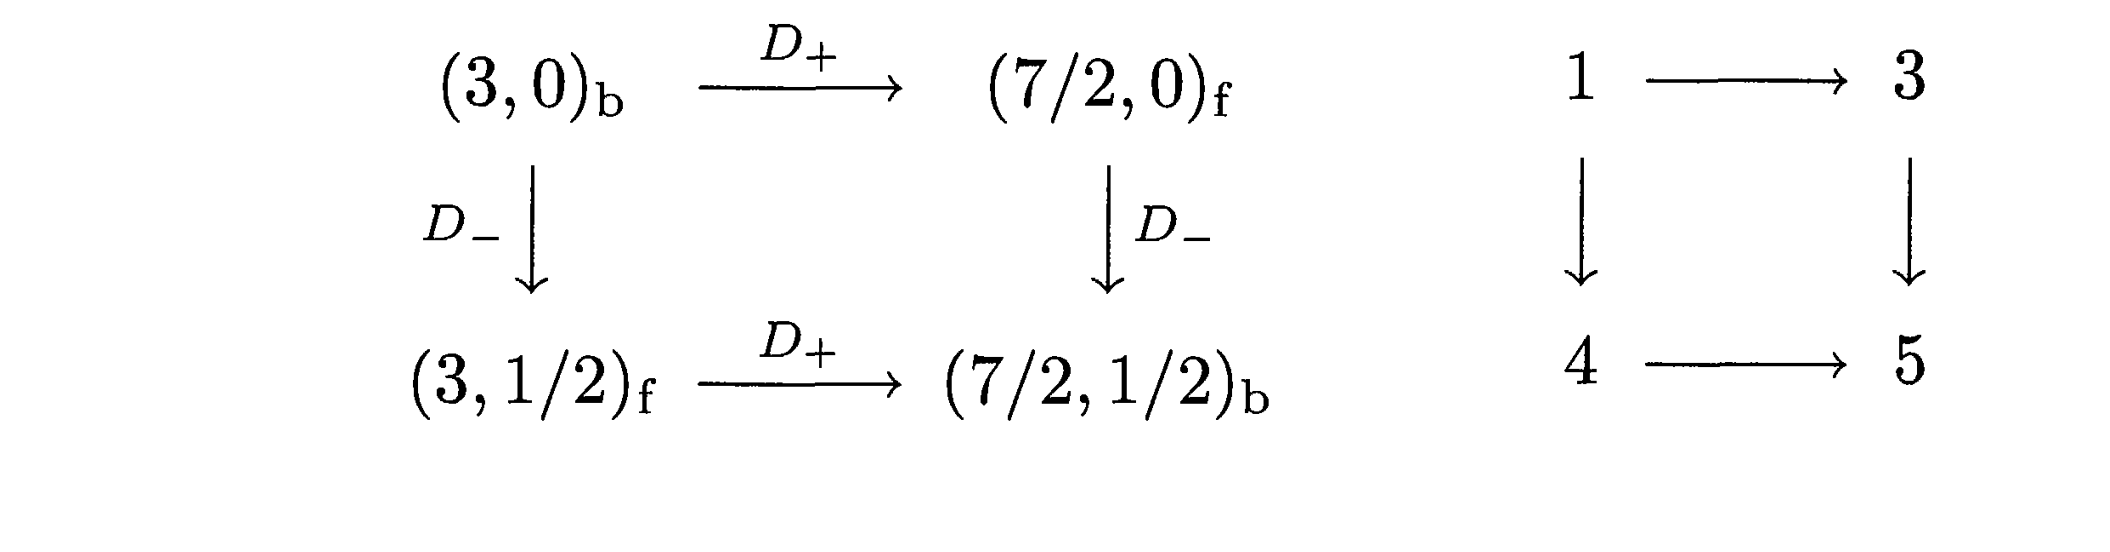
\includegraphics[width=0.86\textwidth]{figs/fig_p296_1.png}
  \caption{算符空间之间的 $D_\pm$ 作用与各空间维数。左：$(3,0)_{\mathrm b}\xrightarrow{D_+}(7/2,0)_{\mathrm f}$、$(3,1/2)_{\mathrm f}\xrightarrow{D_+}(7/2,1/2)_{\mathrm b}$，以及沿 $D_-$ 方向的竖直箭头；右：相应空间维数 $1\to3$、$4\to5$。（原文 Figure，未编号，p.296）}
  \label{fig:p296-1}
\end{figure}

% ===== 原文 p.297 =====
由量纲计数（与 §4.3 中相同）可知，我们可以取所需的 $\mathscr{X}_+$ 具有双分次 $(7/2,0)$，$\mathscr{X}_-$ 具有双分次 $(3,1/2)$。然后计算 $\mathcal{J}$ 的权重，从而得到相应守恒荷 $Q$ 的权重，结果是 $[K,Q]=3Q$，其中 $K$ 是 Lorentz 助推（Lorentz boost）。所以 $Q$ 不与 Poincaré 对易，这正是我们所要的。

\subsection*{问题 5 的解答}

（a）这个模型有两个玻色场：一个映射 $\phi\colon\mathbb{R}^2\to\mathbb{R}^{n+1}$，以及一个「Lagrange 乘子」$\sigma\colon\mathbb{R}^2\to\mathbb{R}$。作用量为
\[
\mathcal{L}=\frac{1}{2\lambda}|d\phi|^2-\frac{i\sigma}{2}(|\phi|^2-1).
\]
容易算出经典运动方程
\[
\begin{aligned}
|\phi|^2&=1\\
\frac{\Delta}{\lambda}\phi&=i\sigma\phi .
\end{aligned}
\]
我们的 Laplacian「$\Delta$」是非负的。第一个方程说明 $\phi$ 映入 $n$ 维球面 $S^n$，第二个说明 $\phi$ 的 Laplacian 垂直于 $S^n$。这意味着 $\phi$ 是到 $S^n$ 的调和映射（harmonic map）。我们把 $\sigma$ 用 $\phi$ 表示为
\begin{equation}
  \sigma=\frac{1}{i\lambda}(\Delta\phi,\phi).
  \tag{5.1}
  \label{eq:sol5-1}
\end{equation}
差一个全导数，$\sigma=\frac{1}{i\lambda}|d\phi|^2$。

（b）按照方程 (5.1)，$\sigma$ 场的量纲为 2，因为 $\phi$ 是二维中的标量场、量纲为 0。我们预期两点函数在位置空间中的行为是
\[
\langle\sigma(x)\sigma(0)\rangle\sim\frac{1}{|x|^4}\qquad\text{当 }x\to0,
\]
等价地，在动量空间中的行为是
\begin{equation}
  \langle\sigma(q)\sigma(-q)\rangle\sim q^2\qquad\text{当 }q\to\infty,
  \tag{5.2}
  \label{eq:sol5-2}
\end{equation}
其中可能有源于反常维数（anomalous dimension）的对数修正。我们可以先把 $\sigma$ 场积掉，从而得到到 $S^n$ 的 $\sigma$ 模型；由于这个理论是渐近自由的（asymptotically free），$|d\phi|^2$ 的两点函数确实呈现 (5.2) 的行为（相差对数修正）。这里我们反过来做：先积掉 $\phi$，计算 $\sigma$ 的有效作用量，至少在大 $n$ 极限下。

有效作用量的计算出现在本讲义 §4.2：
\begin{equation}
  \Gamma(\tilde\sigma)=\frac{n}{2}\left\{\operatorname{Tr}\ln(\Delta-i\tilde\sigma\tilde\lambda)+i\tilde\sigma\right\}.
  \tag{5.3}
  \label{eq:sol5-3}
\end{equation}
其中 $\tilde\sigma=\sigma/n$，$\tilde\lambda=\lambda n$。我们知道应当围绕值 $-i\tilde\sigma_0\tilde\lambda=M^2$（$M^2$ 为正常数）展开。$\tilde\sigma$ 传播子（propagator）是作用量 (5.3) 的

% ===== 原文 p.298 =====
二阶导数，我们在常数 $\tilde\sigma_0=iM^2/\tilde\lambda$ 处取值：
\begin{align}
\left.\frac{\delta^2\Gamma}{\delta\tilde\sigma^2}\right|_{\tilde\sigma_0}
&=\frac{n\tilde\lambda^2}{2}\operatorname{Tr}\left((\Delta+M^2)^{-1}\delta\tilde\sigma\,(\Delta+M^2)^{-1}\delta\tilde\sigma\right)\notag\\
&=\frac{n\tilde\lambda^2}{2}\int dx\,dy\,G(x,y)\,\delta\tilde\sigma(y)\,G(y,x)\,\delta\tilde\sigma(x)\tag{5.4}\label{eq:sol5-4}\\
&=\frac{n\tilde\lambda^2}{2}\int dx\,dy\,G(x,y)^2\,\delta\tilde\sigma(x)\,\delta\tilde\sigma(y),\notag
\end{align}
其中 $G$ 是 Green 函数 $(\Delta+M^2)^{-1}$ 的核。于是 $\tilde\sigma$ 的逆传播子的核为 $\frac{n\tilde\lambda^2}{2}G(x,y)^2$。在动量空间中，平方变为卷积（convolution），于是 $\tilde\sigma$ 逆传播子的核为
\begin{align}
K(q,-q)&=\frac{n\tilde\lambda^2}{2}\int\frac{d^2p}{(2\pi)^2}\,\frac{1}{p^2+M^2}\,\frac{1}{(q-p)^2+M^2}\notag\\
&=\frac{n\tilde\lambda^2}{8\pi^2}\int_0^1 d\alpha\int d^2p\,\frac{1}{[p^2+M^2+\alpha(1-\alpha)q^2]^2}\notag\\
&=\frac{n\tilde\lambda^2}{8\pi}\int_0^1\frac{d\alpha}{M^2+\alpha(1-\alpha)q^2}\tag{5.5}\label{eq:sol5-5}\\
&=\frac{n\tilde\lambda^2}{4\pi}\,\frac{\ln\left(\dfrac{\sqrt{1+4M^2/q^2}+1}{\sqrt{1+4M^2/q^2}-1}\right)}{q^2\sqrt{1+4M^2/q^2}}\notag\\
&\sim\frac{n\tilde\lambda^2}{2\pi}\,\frac{\ln(q^2/M^2)}{q^2}\qquad\text{当 }q\to\infty .\notag
\end{align}

% [Tutor Note: 由第二行到第三行用了二维的 Feynman 参数化与积分 $\int\frac{d^2p}{(2\pi)^2}\frac{1}{(p^2+\Delta)^2}=\frac{1}{4\pi\Delta}$（四维是 $\frac{1}{16\pi^2\Delta}$，最易混错）；把它与 $\frac{n\tilde\lambda^2}{8\pi^2}$ 中的 $(2\pi)^{-2}$ 合并，得到的正是 $\frac{n\tilde\lambda^2}{8\pi}\cdot\frac{1}{\Delta}$，系数中的 $8\pi$（而非 $8\pi^2$）是二维的标志。由第三行到第四行是标准的 $\int_0^1\frac{d\alpha}{M^2+\alpha(1-\alpha)q^2}=\frac{2}{q\sqrt{q^2+4M^2}}\ln\frac{\sqrt{q^2+4M^2}+\sqrt{q^2}}{\sqrt{q^2+4M^2}-\sqrt{q^2}}$；大 $q$ 时它趋于 $\frac{2}{q^2}\ln\frac{q^2}{M^2}$，恰好把 $\frac{1}{4\pi}$ 变成末行的 $\frac{1}{2\pi}$，故末行系数是自洽的。]

于是 $\tilde\sigma$ 传播子的行为是
\[
\langle\tilde\sigma(q)\tilde\sigma(-q)\rangle\sim\frac{2\pi}{n\tilde\lambda^2}\,\frac{q^2}{\ln(q^2/M^2)}\qquad\text{当 }q\to\infty .
\]
由 $\tilde\sigma=\sigma/n$，我们最终得到
\begin{equation}
  \langle\sigma(q)\sigma(-q)\rangle\sim\frac{2\pi n}{\tilde\lambda^2}\,\frac{q^2}{\ln(q^2/M^2)}\qquad\text{当 }q\to\infty .
  \tag{5.6}
  \label{eq:sol5-6}
\end{equation}

注意：对 $n$ 的依赖本可由 (5.1) 预言，因为 $(\Delta\phi,\phi)$ 的两点函数是单个标量场两点函数的 $n+1$ 倍。大 $q$ 的行为正如 (5.2) 所预言，只是被一个对数所修正。

注意：逆传播子 (5.5) 可以用图来计算。把我们的 $\phi$ 积掉所得的有效作用量，由带外 $\sigma$ 线、内 $\phi$ 线的图来计算。当然，我们应当围绕 $\sigma=iM^2/\lambda$ 展开。对二次项只有一个图，如图所示；图中实线代表 $\phi$，点线代表 $\sigma$。注意由于 $\sigma$ 的平移，$\phi$ 的传播子是有质量的。这个图正是由 (5.5) 计算的。

\begin{figure}[htbp]
  \centering
  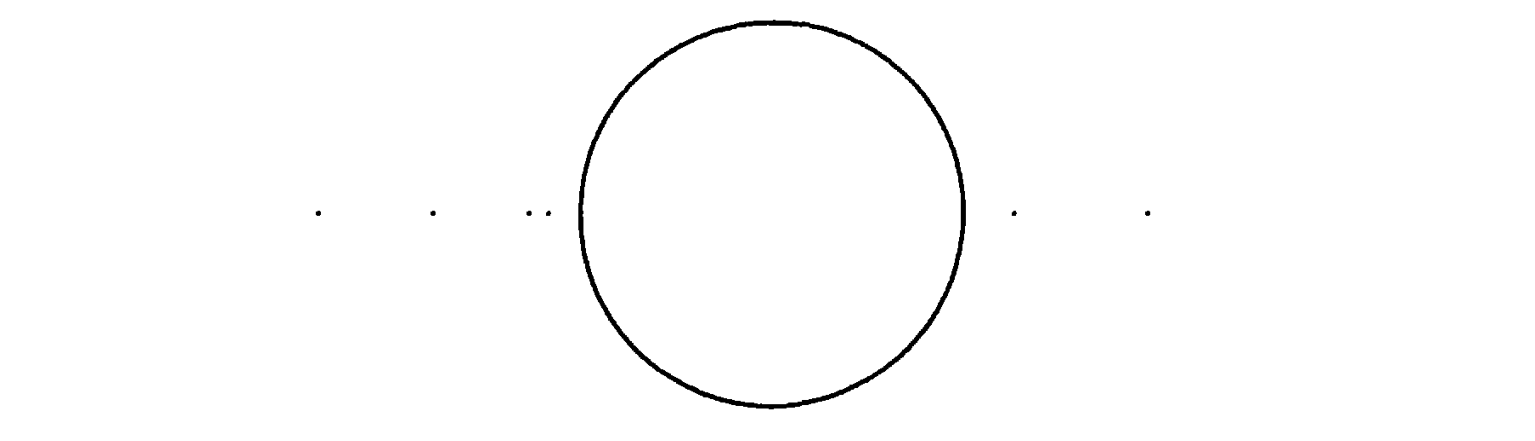
\includegraphics[width=0.55\textwidth]{figs/fig_p298_1.png}
  \caption{二次项的唯一一个图：实线圆环为内 $\phi$ 线，两侧点线为外 $\sigma$ 线。（原文 Figure，未编号，p.298）}
  \label{fig:p298-1}
\end{figure}

% ===== 原文 p.299 =====
\subsection*{问题 10 的解答}

我们沿用 [I-Supersolutions] 的记号与约定。

二维中的手征超场（chiral superfield）$\Phi$ 具有分量场 $\phi,\psi_\pm,\bar\psi_\pm$。以 $K$ 记无穷小旋转生成元，以 $J_-$ 与 $J_+$ 记 R 对称性的无穷小生成元（在第 14 讲中称为 $J_L$ 与 $J_R$）。我们所考虑的拓扑扭曲（topological twist）取 $K-\frac12J_-+\frac12J_+$ 作为欧氏旋转的新的无穷小生成元。下面的表格给出各分量场在这些无穷小对称性下的权重：

\begin{center}
\begin{tabular}{c|cccc}
\hline
分量场 & $K$ & $J_-$ & $J_+$ & $K-\frac12J_-+\frac12J_+$\\
\hline\hline
$\phi$ & $0$ & $0$ & $0$ & $0$\\
$\psi_+$ & $1/2$ & $0$ & $1$ & $1$\\
$\bar\psi_+$ & $1/2$ & $0$ & $-1$ & $0$\\
$\psi_-$ & $-1/2$ & $1$ & $0$ & $-1$\\
$\bar\psi_-$ & $-1/2$ & $-1$ & $0$ & $0$\\
\hline
\end{tabular}
\end{center}

% [Tutor Note: 用最后一列可自检扭曲是否正确：$\bar\psi_+$ 与 $\bar\psi_-$ 的新权重都是 0，故 $\bar\chi=\bar\psi_++\bar\psi_-$ 是 $\Sigma$ 上的标量；$\psi_+$ 权重 $1$、$\psi_-$ 权重 $-1$，分别给出 $(1,0)$ 与 $(0,1)$ 形式——这正是「把超 Riemann 面映到 Kähler 流形」所要求的。易错处有二：其一，$K$ 的归一化（此处旋转生成元在 $\psi_\pm$ 上取 $\pm1/2$，若改用 $\pm1$ 的约定，整列都要乘 2）；其二，$J_\pm$ 的符号，$\bar\psi_+$ 的 $J_+=-1$ 与 $\psi_+$ 的 $J_+=+1$ 差一个符号，若抄错，$\bar\psi_+$ 的新权重会变成 1，$\bar\chi$ 就不再是标量。]

超对称 $\bar Q_++\bar Q_-$ 与新的旋转生成元对易，因此它是扭曲后理论的超对称。

考虑扭曲理论中一个把超 Riemann 面映入 Kähler 流形（Kähler manifold）$X$ 的手征超场。表格的最后一列表明各分量场在底流形 $\Sigma$ 上如何变换。于是 $\phi$ 是从底流形 $\Sigma$ 到 $X$ 的映射，奇场 $\bar\psi_\pm$ 是 $\Sigma$ 上的标量、取值于反全纯切丛 $\phi^*T_{0,1}X$，而奇场 $\psi_+$（相应地 $\psi_-$）是 $\Sigma$ 上的 $(1,0)$ 形式（相应地 $(0,1)$ 形式）、取值于全纯切丛 $\phi^*T_{1,0}X$。定义新的奇场 $\bar\chi$ 与 $\bar\chi'$ 会比较方便：
\begin{equation}
  \begin{aligned}
    \bar\chi&=\bar\psi_++\bar\psi_-,\\
    \bar\chi'&=\bar\psi_+-\bar\psi_- .
  \end{aligned}
  \tag{10.1}
  \label{eq:sol10-1}
\end{equation}

现在我们取目标空间 $X=\mathbb{C}^n$ 这一特殊情形。如本讲义 §14.3.1 所解释的，我们把拓扑期望值的计算归结为对场的最低模（lowest modes）的积分。当 $\Sigma$ 的亏格（genus）为 0 时，不存在全纯的 $(1,0)$ 形式（也不存在反全纯的 $(0,1)$ 形式），因此我们可以消去 $\psi_\pm$。其余场 $\phi,\bar\chi,\bar\chi'$ 都化为常数。对这些常数场，我们用量纲约化 [I-Supersolutions, §5.1] 中最后那些方程的办法来计算超对称变换律。对 $\delta=\bar\eta(\bar Q_++\bar Q_-)$，我们得到
\[
\begin{aligned}
\delta\bar\phi&=-\sqrt2\,\bar\eta\,\bar\chi\\
\delta\bar\chi&=0\\
\delta\bar\chi'&=2\sqrt2\,\bar\eta\,\overline{\operatorname{grad}W(\phi)}.
\end{aligned}
\]

% [Tutor Note: 这三行都是 $\bar Q_++\bar Q_-$ 的变分，作用对象是带上横线的场，故第一行左端是 $\delta\bar\phi$；第三行右端「$\operatorname{grad}W(\phi)$」上方的横线表示对 $\phi$ 取共轭（即 $\partial\bar W/\partial\bar\phi$），不是排印污迹。自洽性检验：$\delta^2\bar\chi'=2\sqrt2\,\bar\eta\,\overline{\operatorname{Hess}W}\cdot\delta\bar\phi\propto\bar\eta^2=0$，故在常数场上 $\delta^2=0$，这正是拓扑（BRST 型）对称性所要求的；若忽略第一行的横线、把 $\phi$ 与 $\bar\phi$ 混为一谈，就会得出 $\delta^2\bar\chi'\neq0$ 的错误结论。]
这些场的 Lagrange 量，由量纲约化 [I-Supersolutions, §5.3] 中的一般 Lagrange 量、限制到常数场、再 Wick 转动到欧氏号差而得到：
\[
L=\|\operatorname{grad}W(\phi)\|^2-\frac12\operatorname{Hess}\overline{W}(\phi)(\bar\chi',\bar\chi).
\]
